%---------------------------------------------------------------------------------------
% Configuracion de Documento
%---------------------------------------------------------------------------------------
\documentclass[10pt, a4paper,english]{article}

\parindent=20pt
\parskip=1pt
\usepackage[width=15.5cm, left=3cm, top=2cm, height= 24.5cm]{geometry}

% User package
\usepackage{epigraph}
\usepackage{amsmath}
\usepackage{amsfonts}
\usepackage{amssymb}
\usepackage{fancyhdr}
\usepackage[activeacute, spanish]{babel}
\usepackage{cancel}
\usepackage[utf8]{inputenc}
%\usepackage{graphicx}
\usepackage{algorithm}
%\usepackage{algorithmic}
%\usepackage{algorithm2e}
\usepackage{algpseudocode}
%\usepackage{afterpage}
\usepackage{lastpage}
\usepackage{listings}
\usepackage{url}
\usepackage{mathptmx}
\usepackage{cite}
\usepackage{pifont}
\usepackage{float}
\usepackage{color}     % para snipets de codigo coloreados
\usepackage{xcolor}
\usepackage{fancybox}  % para el sbox de los snipets de codigo
\usepackage[pdftex]{graphicx}
\usepackage{graphicx} %paquete para incluir imagenes
\usepackage{caption}
\usepackage{subcaption}




\lstset{frame=tb,
	  language=Java,
	  aboveskip=3mm,
	  belowskip=3mm,
	  showstringspaces=false,
	  columns=flexible,
	  basicstyle={\scriptsize\ttfamily},
	  numberstyle=\tiny\color{gray},
	  keywordstyle=\color{blue},
	  commentstyle=\color{green},
	  stringstyle=\color{red},
	  breaklines=true,
	  breakatwhitespace=true,
	  tabsize=3,
	  numbers=left,
	  numbersep=15pt,
	  numberfirstline = false
	}


\pagestyle{fancy}

\thispagestyle{fancy}

\addtolength{\headheight}{1pt}

\lhead{Udacity Isolation Project}

\rhead{Omar Ghaleb} % <--- Cambiar de acuerdo al tp actual

\cfoot{\thepage /\pageref{LastPage}}

\renewcommand{\footrulewidth}{0.4pt}

% Informacion del documento

\author{\normalsize{Omar Ghaleb}}

\date{\normalsize{February 14th, 2017}} % <--- Cambiar de acuerdo al tp actual

\title{
%	\includegraphics[width=0.05\textwidth]{udacity-small.png}\\
Build a Game-Playing Agent for the Isolation Game \\
\large {Research Review}
} % <--- Cambiar de acuerdo al tp actual


\begin{document}

\begin{center}

%\includegraphics[width=0.05\textwidth]{udacity-small.png}\\
Build a Game-Playing Agent: Heuristic Analysis \\
Omar Ghaleb \\
\end{center}

\section{Introduction}

This paper will present three evaluation functions or heuristics for winning the isolation game. The evaluation is based on the tournament performance.
%This summary presents three evaluation functions to winning the Isolation Game.\\ 
%
%Each heuristic idea is evaluated separately and compared to ID\_Improved evaluation function. At the end, a fourth heuristic, combining some of those ideas, is analyzed and presented as final heuristic.\\

\section{Heuristics}

\subsection{Heuristic 1: Agent moves vs. opponent moves}

%\subsubsection{Definition}

The $ID\_Improved$ heuristic uses the function:
	$$score = my\_moves - opponent\_moves$$

%As we saw in the course, this metric could be improved assigning weight to each element. We can define a new evaluation function as:
This evaluation function can be improved by assigning weights to the opponents moves or my moves, so we assigned weights to the opponents moves to give more weight to the moves available that gives the opponents less moves. The new function:
	$$score = my\_moves - 3*opponent\_moves$$

The weight value can be different and we can change how early the cutoff of the tree is, but in this we will just use one value which is $3$.

\subsection{Heuristic 2: Agent position vs. opponent position}


This evaluation function uses the position of the agent and the opponent to evaluate the moves available for the agent. The moves that distance the agent from the opponent gets a higher score better than the one that keeps him closer. The evaluation function is as follow:
	$$score = my\_position - opponent\_position$$

\subsection{Heuristic 3: Using both the position and number of moves}


This heuristic uses both the first and the second heuristic to improve the score function. This allows the agent to take into consideration the number of moves available for it and at the same time, evaluating them according to the distance from the opponent. The function is as follows:
	$$distance = my\_position - opponent\_position$$
	$$score = (my\_moves + distance) - 3*opponent\_moves$$


\subsection{Results}

To evaluate the performance of the heuristic, the tournament was used to compare the win rate. In the results, $AB\_custom$ is H3 which uses the combination of H1 and H2. $AB\_custom\_2$ is H2. $AB\_custom\_3$ is H1.

The performance rates obtained are shown in this graph:


\begin{center}
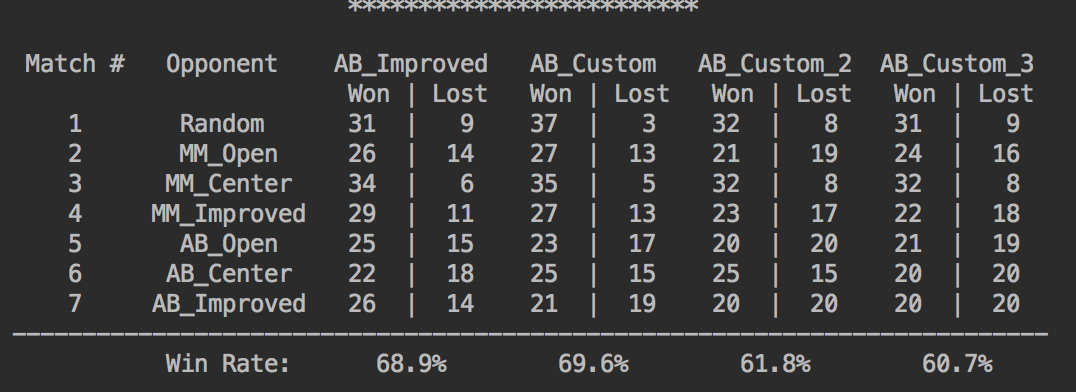
\includegraphics[width=0.8\textwidth]{isolation-results.png}\\
\end{center}

In the graph, we can see that the mixed heuristic, which is $AB\_custom$, outperforms the other two heuristics by almost 9\% increase in the win rate. In $AB\_custom\_2$, which is using only the number of moves, the win rate is 61.8\%. And in $AB\_custom\_3$, which uses the position of the agent and the opponent, the win rate is even lower with 60.7\%. After combining both to create the first heuristic $AB\_custom$, we can see a huge increase in the win rate to obtain a 69.6\% win rate.

\section{Conclusion}

In this report, three heuristics were introduced:

\begin{itemize}
\item \textbf{My Moves vs Opponent Moves:} that shows better performance than ID\_Improved sometimes. 
\item \textbf{My Position vs Opponent Position:} This uses the distance between the two players to evaluate a move.
\item \textbf{Mixed:} This uses both the first and second heuristics.
\end{itemize}

From the results, we can see that the mixed heuristic is the recommended one according to the following reasons:

\begin{itemize}
  \item It is built on the bases of the number of moves which is considered already a good heuristic.
  \item Using a weight will make the agent make aggressive to cut the search trees as early as possible.
  \item The results obtained in experimentation shows a better performance against \textit{ID\_Improved}
  \item Mixing both the moves and the positions heuristics, make use of the advantages of both.
\end{itemize}


Due to randomness, sometimes the results fluctuate being better or worse than $AB\_improved$.


% \section{Appendix}

% \subsection{My moves vs opponent moves run results}

% \begin{lstlisting}

% *************************
% Evaluating: Student MyMovesVsOpponent0
% *************************

% Playing Matches:
% ----------
%   Match 1: Student MyMovesVsOpponent0 vs   Random    	Result: 153 to 7
%   Match 2: Student MyMovesVsOpponent0 vs   MM\_Null   	Result: 153 to 7
%   Match 3: Student MyMovesVsOpponent0 vs   MM\_Open   	Result: 124 to 36
%   Match 4: Student MyMovesVsOpponent0 vs MM\_Improved 	Result: 104 to 56
%   Match 5: Student MyMovesVsOpponent0 vs   AB\_Null   	Result: 132 to 28
%   Match 6: Student MyMovesVsOpponent0 vs   AB\_Open   	Result: 95 to 65
%   Match 7: Student MyMovesVsOpponent0 vs AB\_Improved 	Result: 90 to 70


% Results:
% ----------
% Student MyMovesVsOpponent0     75.98%

% *************************
% Evaluating: Student MyMovesVsOpponent0.5
% *************************

% Playing Matches:
% ----------
%   Match 1: Student MyMovesVsOpponent0.5 vs   Random    	Result: 150 to 10
%   Match 2: Student MyMovesVsOpponent0.5 vs   MM\_Null   	Result: 154 to 6
%   Match 3: Student MyMovesVsOpponent0.5 vs   MM\_Open   	Result: 119 to 41
%   Match 4: Student MyMovesVsOpponent0.5 vs MM\_Improved 	Result: 115 to 45
%   Match 5: Student MyMovesVsOpponent0.5 vs   AB\_Null   	Result: 133 to 27
%   Match 6: Student MyMovesVsOpponent0.5 vs   AB\_Open   	Result: 102 to 58
%   Match 7: Student MyMovesVsOpponent0.5 vs AB\_Improved 	Result: 92 to 68


% Results:
% ----------
% Student MyMovesVsOpponent0.5     77.23%

% *************************
% Evaluating: Student MyMovesVsOpponent1
% *************************

% Playing Matches:
% ----------
%   Match 1: Student MyMovesVsOpponent1 vs   Random    	Result: 156 to 4
%   Match 2: Student MyMovesVsOpponent1 vs   MM\_Null   	Result: 147 to 13
%   Match 3: Student MyMovesVsOpponent1 vs   MM\_Open   	Result: 120 to 40
%   Match 4: Student MyMovesVsOpponent1 vs MM\_Improved 	Result: 110 to 50
%   Match 5: Student MyMovesVsOpponent1 vs   AB\_Null   	Result: 140 to 20
%   Match 6: Student MyMovesVsOpponent1 vs   AB\_Open   	Result: 115 to 45
%   Match 7: Student MyMovesVsOpponent1 vs AB\_Improved 	Result: 101 to 59


% Results:
% ----------
% Student MyMovesVsOpponent1     79.38%

% *************************
% Evaluating: Student MyMovesVsOpponent1.5
% *************************

% Playing Matches:
% ----------
%   Match 1: Student MyMovesVsOpponent1.5 vs   Random    	Result: 157 to 3
%   Match 2: Student MyMovesVsOpponent1.5 vs   MM\_Null   	Result: 156 to 4
%   Match 3: Student MyMovesVsOpponent1.5 vs   MM\_Open   	Result: 127 to 33
%   Match 4: Student MyMovesVsOpponent1.5 vs MM\_Improved 	Result: 115 to 45
%   Match 5: Student MyMovesVsOpponent1.5 vs   AB\_Null   	Result: 141 to 19
%   Match 6: Student MyMovesVsOpponent1.5 vs   AB\_Open   	Result: 106 to 54
%   Match 7: Student MyMovesVsOpponent1.5 vs AB\_Improved 	Result: 98 to 62


% Results:
% ----------
% Student MyMovesVsOpponent1.5     80.36%

% *************************
% Evaluating: Student MyMovesVsOpponent2
% *************************

% Playing Matches:
% ----------
%   Match 1: Student MyMovesVsOpponent2 vs   Random    	Result: 158 to 2
%   Match 2: Student MyMovesVsOpponent2 vs   MM\_Null   	Result: 154 to 6
%   Match 3: Student MyMovesVsOpponent2 vs   MM\_Open   	Result: 120 to 40
%   Match 4: Student MyMovesVsOpponent2 vs MM\_Improved 	Result: 115 to 45
%   Match 5: Student MyMovesVsOpponent2 vs   AB\_Null   	Result: 134 to 26
%   Match 6: Student MyMovesVsOpponent2 vs   AB\_Open   	Result: 116 to 44
%   Match 7: Student MyMovesVsOpponent2 vs AB\_Improved 	Result: 100 to 60


% Results:
% ----------
% Student MyMovesVsOpponent2     80.09%

% *************************
% Evaluating: Student MyMovesVsOpponent2.5
% *************************

% Playing Matches:
% ----------
%   Match 1: Student MyMovesVsOpponent2.5 vs   Random    	Result: 156 to 4
%   Match 2: Student MyMovesVsOpponent2.5 vs   MM\_Null   	Result: 146 to 14
%   Match 3: Student MyMovesVsOpponent2.5 vs   MM\_Open   	Result: 123 to 37
%   Match 4: Student MyMovesVsOpponent2.5 vs MM\_Improved 	Result: 118 to 42
%   Match 5: Student MyMovesVsOpponent2.5 vs   AB\_Null   	Result: 138 to 22
%   Match 6: Student MyMovesVsOpponent2.5 vs   AB\_Open   	Result: 113 to 47
%   Match 7: Student MyMovesVsOpponent2.5 vs AB\_Improved 	Result: 97 to 63


% Results:
% ----------
% Student MyMovesVsOpponent2.5     79.55%

% *************************
% Evaluating: Student MyMovesVsOpponent3
% *************************

% Playing Matches:
% ----------
%   Match 1: Student MyMovesVsOpponent3 vs   Random    	Result: 147 to 13
%   Match 2: Student MyMovesVsOpponent3 vs   MM\_Null   	Result: 149 to 11
%   Match 3: Student MyMovesVsOpponent3 vs   MM\_Open   	Result: 125 to 35
%   Match 4: Student MyMovesVsOpponent3 vs MM\_Improved 	Result: 125 to 35
%   Match 5: Student MyMovesVsOpponent3 vs   AB\_Null   	Result: 145 to 15
%   Match 6: Student MyMovesVsOpponent3 vs   AB\_Open   	Result: 118 to 42
%   Match 7: Student MyMovesVsOpponent3 vs AB\_Improved 	Result: 105 to 55


% Results:
% ----------
% Student MyMovesVsOpponent3     81.61%

% *************************
% Evaluating: Student MyMovesVsOpponent3.5
% *************************

% Playing Matches:
% ----------
%   Match 1: Student MyMovesVsOpponent3.5 vs   Random    	Result: 154 to 6
%   Match 2: Student MyMovesVsOpponent3.5 vs   MM\_Null   	Result: 153 to 7
%   Match 3: Student MyMovesVsOpponent3.5 vs   MM\_Open   	Result: 125 to 35
%   Match 4: Student MyMovesVsOpponent3.5 vs MM\_Improved 	Result: 120 to 40
%   Match 5: Student MyMovesVsOpponent3.5 vs   AB\_Null   	Result: 145 to 15
%   Match 6: Student MyMovesVsOpponent3.5 vs   AB\_Open   	Result: 108 to 52
%   Match 7: Student MyMovesVsOpponent3.5 vs AB\_Improved 	Result: 99 to 61


% Results:
% ----------
% Student MyMovesVsOpponent3.5     80.71%

% *************************
% Evaluating: Student MyMovesVsOpponent4
% *************************

% Playing Matches:
% ----------
%   Match 1: Student MyMovesVsOpponent4 vs   Random    	Result: 157 to 3
%   Match 2: Student MyMovesVsOpponent4 vs   MM\_Null   	Result: 154 to 6
%   Match 3: Student MyMovesVsOpponent4 vs   MM\_Open   	Result: 129 to 31
%   Match 4: Student MyMovesVsOpponent4 vs MM\_Improved 	Result: 117 to 43
%   Match 5: Student MyMovesVsOpponent4 vs   AB\_Null   	Result: 132 to 28
%   Match 6: Student MyMovesVsOpponent4 vs   AB\_Open   	Result: 112 to 48
%   Match 7: Student MyMovesVsOpponent4 vs AB\_Improved 	Result: 93 to 67


% Results:
% ----------
% Student MyMovesVsOpponent4     79.82%

% *************************
% Evaluating: Student MyMovesVsOpponent4.5
% *************************

% Playing Matches:
% ----------
%   Match 1: Student MyMovesVsOpponent4.5 vs   Random    	Result: 151 to 9
%   Match 2: Student MyMovesVsOpponent4.5 vs   MM\_Null   	Result: 147 to 13
%   Match 3: Student MyMovesVsOpponent4.5 vs   MM\_Open   	Result: 124 to 36
%   Match 4: Student MyMovesVsOpponent4.5 vs MM\_Improved 	Result: 115 to 45
%   Match 5: Student MyMovesVsOpponent4.5 vs   AB\_Null   	Result: 142 to 18
%   Match 6: Student MyMovesVsOpponent4.5 vs   AB\_Open   	Result: 111 to 49
%   Match 7: Student MyMovesVsOpponent4.5 vs AB\_Improved 	Result: 98 to 62


% Results:
% ----------
% Student MyMovesVsOpponent4.5     79.29%

% *************************
% Evaluating: Student MyMovesVsOpponent5
% *************************

% Playing Matches:
% ----------
%   Match 1: Student MyMovesVsOpponent5 vs   Random    	Result: 155 to 5
%   Match 2: Student MyMovesVsOpponent5 vs   MM\_Null   	Result: 150 to 10
%   Match 3: Student MyMovesVsOpponent5 vs   MM\_Open   	Result: 118 to 42
%   Match 4: Student MyMovesVsOpponent5 vs MM\_Improved 	Result: 123 to 37
%   Match 5: Student MyMovesVsOpponent5 vs   AB\_Null   	Result: 136 to 24
%   Match 6: Student MyMovesVsOpponent5 vs   AB\_Open   	Result: 107 to 53
%   Match 7: Student MyMovesVsOpponent5 vs AB\_Improved 	Result: 104 to 56


% Results:
% ----------
% Student MyMovesVsOpponent5     79.73%

% *************************
% Evaluating: Student MyMovesVsOpponent5.5
% *************************

% Playing Matches:
% ----------
%   Match 1: Student MyMovesVsOpponent5.5 vs   Random    	Result: 156 to 4
%   Match 2: Student MyMovesVsOpponent5.5 vs   MM\_Null   	Result: 147 to 13
%   Match 3: Student MyMovesVsOpponent5.5 vs   MM\_Open   	Result: 122 to 38
%   Match 4: Student MyMovesVsOpponent5.5 vs MM\_Improved 	Result: 119 to 41
%   Match 5: Student MyMovesVsOpponent5.5 vs   AB\_Null   	Result: 140 to 20
%   Match 6: Student MyMovesVsOpponent5.5 vs   AB\_Open   	Result: 107 to 53
%   Match 7: Student MyMovesVsOpponent5.5 vs AB\_Improved 	Result: 96 to 64


% Results:
% ----------
% Student MyMovesVsOpponent5.5     79.20%
% \end{lstlisting}


% \subsection{Center Opening}
% \begin{lstlisting}
% *************************
% Evaluating: Student GameStart
% *************************

% Playing Matches:
% ----------
%   Match 1: Student GameStart vs   Random    	Result: 155 to 5
%   Match 2: Student GameStart vs   MM_Null   	Result: 145 to 15
%   Match 3: Student GameStart vs   MM_Open   	Result: 130 to 30
%   Match 4: Student GameStart vs MM_Improved 	Result: 123 to 37
%   Match 5: Student GameStart vs   AB_Null   	Result: 134 to 26
%   Match 6: Student GameStart vs   AB_Open   	Result: 102 to 58
%   Match 7: Student GameStart vs AB_Improved 	Result: 101 to 59


% Results:
% ----------
% Student GameStart  2   79.46%

% *************************
% Evaluating: Student GameStart
% *************************

% Playing Matches:
% ----------
%   Match 1: Student GameStart vs   Random    	Result: 158 to 2
%   Match 2: Student GameStart vs   MM_Null   	Result: 148 to 12
%   Match 3: Student GameStart vs   MM_Open   	Result: 124 to 36
%   Match 4: Student GameStart vs MM_Improved 	Result: 116 to 44
%   Match 5: Student GameStart vs   AB_Null   	Result: 144 to 16
%   Match 6: Student GameStart vs   AB_Open   	Result: 107 to 53
%   Match 7: Student GameStart vs AB_Improved 	Result: 103 to 57


% Results:
% ----------
% Student GameStart  3   80.36%

% *************************
% Evaluating: Student GameStart
% *************************

% Playing Matches:
% ----------
%   Match 1: Student GameStart vs   Random    	Result: 154 to 6
%   Match 2: Student GameStart vs   MM_Null   	Result: 151 to 9
%   Match 3: Student GameStart vs   MM_Open   	Result: 123 to 37
%   Match 4: Student GameStart vs MM_Improved 	Result: 114 to 46
%   Match 5: Student GameStart vs   AB_Null   	Result: 136 to 24
%   Match 6: Student GameStart vs   AB_Open   	Result: 105 to 55
%   Match 7: Student GameStart vs AB_Improved 	Result: 101 to 59


% Results:
% ----------
% Student GameStart  4   78.93%

% *************************
% Evaluating: Student GameStart
% *************************

% Playing Matches:
% ----------
%   Match 1: Student GameStart vs   Random    	Result: 155 to 5
%   Match 2: Student GameStart vs   MM_Null   	Result: 149 to 11
%   Match 3: Student GameStart vs   MM_Open   	Result: 129 to 31
%   Match 4: Student GameStart vs MM_Improved 	Result: 115 to 45
%   Match 5: Student GameStart vs   AB_Null   	Result: 140 to 20
%   Match 6: Student GameStart vs   AB_Open   	Result: 116 to 44
%   Match 7: Student GameStart vs AB_Improved 	Result: 105 to 55


% Results:
% ----------
% Student GameStart   5  81.16%

% *************************
% Evaluating: Student GameStart
% *************************

% Playing Matches:
% ----------
%   Match 1: Student GameStart vs   Random    	Result: 154 to 6
%   Match 2: Student GameStart vs   MM_Null   	Result: 150 to 10
%   Match 3: Student GameStart vs   MM_Open   	Result: 120 to 40
%   Match 4: Student GameStart vs MM_Improved 	Result: 114 to 46
%   Match 5: Student GameStart vs   AB_Null   	Result: 143 to 17
%   Match 6: Student GameStart vs   AB_Open   	Result: 106 to 54
%   Match 7: Student GameStart vs AB_Improved 	Result: 102 to 58


% Results:
% ----------
% Student GameStart  6   79.38%

% *************************
% Evaluating: Student GameStart
% *************************

% Playing Matches:
% ----------
%   Match 1: Student GameStart vs   Random    	Result: 154 to 6
%   Match 2: Student GameStart vs   MM_Null   	Result: 152 to 8
%   Match 3: Student GameStart vs   MM_Open   	Result: 124 to 36
%   Match 4: Student GameStart vs MM_Improved 	Result: 121 to 39
%   Match 5: Student GameStart vs   AB_Null   	Result: 145 to 15
%   Match 6: Student GameStart vs   AB_Open   	Result: 110 to 50
%   Match 7: Student GameStart vs AB_Improved 	Result: 99 to 61


% Results:
% ----------
% Student GameStart    7 80.80%

% Process finished with exit code 0
% \end{lstlisting}

% \subsection{Common Moves}
% \begin{lstlisting}
% *************************
% Evaluating: Student CommonMoves 1
% *************************

% Playing Matches:
% ----------
%   Match 1: Student CommonMoves 1 vs   Random    	Result: 386 to 14
%   Match 2: Student CommonMoves 1 vs   MM_Null   	Result: 366 to 34
%   Match 3: Student CommonMoves 1 vs   MM_Open   	Result: 301 to 99
%   Match 4: Student CommonMoves 1 vs MM_Improved 	Result: 280 to 120
%   Match 5: Student CommonMoves 1 vs   AB_Null   	Result: 332 to 68
%   Match 6: Student CommonMoves 1 vs   AB_Open   	Result: 264 to 136
%   Match 7: Student CommonMoves 1 vs AB_Improved 	Result: 245 to 155


% Results:
% ----------
% Student CommonMoves 1     77.64%

% *************************
% Evaluating: Student CommonMoves 2
% *************************

% Playing Matches:
% ----------
%   Match 1: Student CommonMoves 2 vs   Random    	Result: 384 to 16
%   Match 2: Student CommonMoves 2 vs   MM_Null   	Result: 364 to 36
%   Match 3: Student CommonMoves 2 vs   MM_Open   	Result: 257 to 143
%   Match 4: Student CommonMoves 2 vs MM_Improved 	Result: 259 to 141
%   Match 5: Student CommonMoves 2 vs   AB_Null   	Result: 337 to 63
%   Match 6: Student CommonMoves 2 vs   AB_Open   	Result: 260 to 140
%   Match 7: Student CommonMoves 2 vs AB_Improved 	Result: 235 to 165


% Results:
% ----------
% Student CommonMoves 2     74.86%

% *************************
% Evaluating: Student CommonMoves 3
% *************************

% Playing Matches:
% ----------
%   Match 1: Student CommonMoves 3 vs   Random    	Result: 379 to 21
%   Match 2: Student CommonMoves 3 vs   MM_Null   	Result: 364 to 36
%   Match 3: Student CommonMoves 3 vs   MM_Open   	Result: 261 to 139
%   Match 4: Student CommonMoves 3 vs MM_Improved 	Result: 247 to 153
%   Match 5: Student CommonMoves 3 vs   AB_Null   	Result: 332 to 68
%   Match 6: Student CommonMoves 3 vs   AB_Open   	Result: 239 to 161
%   Match 7: Student CommonMoves 3 vs AB_Improved 	Result: 223 to 177


% Results:
% ----------
% Student CommonMoves 3     73.04%

% Process finished with exit code 0

% *************************
% Evaluating: Student CommonMoves 1
% *************************

% Playing Matches:
% ----------
%   Match 1: Student CommonMoves 1 vs   Random    	Result: 97 to 3
%   Match 2: Student CommonMoves 1 vs   MM_Null   	Result: 98 to 2
%   Match 3: Student CommonMoves 1 vs   MM_Open   	Result: 76 to 24
%   Match 4: Student CommonMoves 1 vs MM_Improved 	Result: 69 to 31
%   Match 5: Student CommonMoves 1 vs   AB_Null   	Result: 88 to 12
%   Match 6: Student CommonMoves 1 vs   AB_Open   	Result: 71 to 29
%   Match 7: Student CommonMoves 1 vs AB_Improved 	Result: 65 to 35


% Results:
% ----------
% Student CommonMoves -1     80.57%

% *************************
% Evaluating: Student CommonMoves 2
% *************************

% Playing Matches:
% ----------
%   Match 1: Student CommonMoves 2 vs   Random    	Result: 94 to 6
%   Match 2: Student CommonMoves 2 vs   MM_Null   	Result: 91 to 9
%   Match 3: Student CommonMoves 2 vs   MM_Open   	Result: 71 to 29
%   Match 4: Student CommonMoves 2 vs MM_Improved 	Result: 74 to 26
%   Match 5: Student CommonMoves 2 vs   AB_Null   	Result: 85 to 15
%   Match 6: Student CommonMoves 2 vs   AB_Open   	Result: 73 to 27
%   Match 7: Student CommonMoves 2 vs AB_Improved 	Result: 64 to 36


% Results:
% ----------
% Student CommonMoves -2     78.86%

% *************************
% Evaluating: Student CommonMoves 3
% *************************

% Playing Matches:
% ----------
%   Match 1: Student CommonMoves 3 vs   Random    	Result: 96 to 4
%   Match 2: Student CommonMoves 3 vs   MM_Null   	Result: 95 to 5
%   Match 3: Student CommonMoves 3 vs   MM_Open   	Result: 78 to 22
%   Match 4: Student CommonMoves 3 vs MM_Improved 	Result: 72 to 28
%   Match 5: Student CommonMoves 3 vs   AB_Null   	Result: 89 to 11
%   Match 6: Student CommonMoves 3 vs   AB_Open   	Result: 71 to 29
%   Match 7: Student CommonMoves 3 vs AB_Improved 	Result: 64 to 36


% Results:
% ----------
% Student CommonMoves -3     80.71%



% \end{lstlisting}


\end{document}
